\chapter{Personal}\label{personal}
Im Kopf des Fensters kann eingestellt werden welche Personen angezeigt werden sollen.
Ebenso kann durch einen Knopfdruck eine E-Mail an alle angezeigten Personen erstellt werden.
Werden bei dieser Aktion Personen gefunden, für die kein Mailadresse angegeben ist,
so können die angegebenen Postadressen in einer CSV-Datei gespeichert werden.
Diese Daten können dann z.B.\ für Serienbriefe genutzt werden.

\section{Gesamtübersicht}\label{personal:gesamtansicht}
\begin{figure}[!h]
	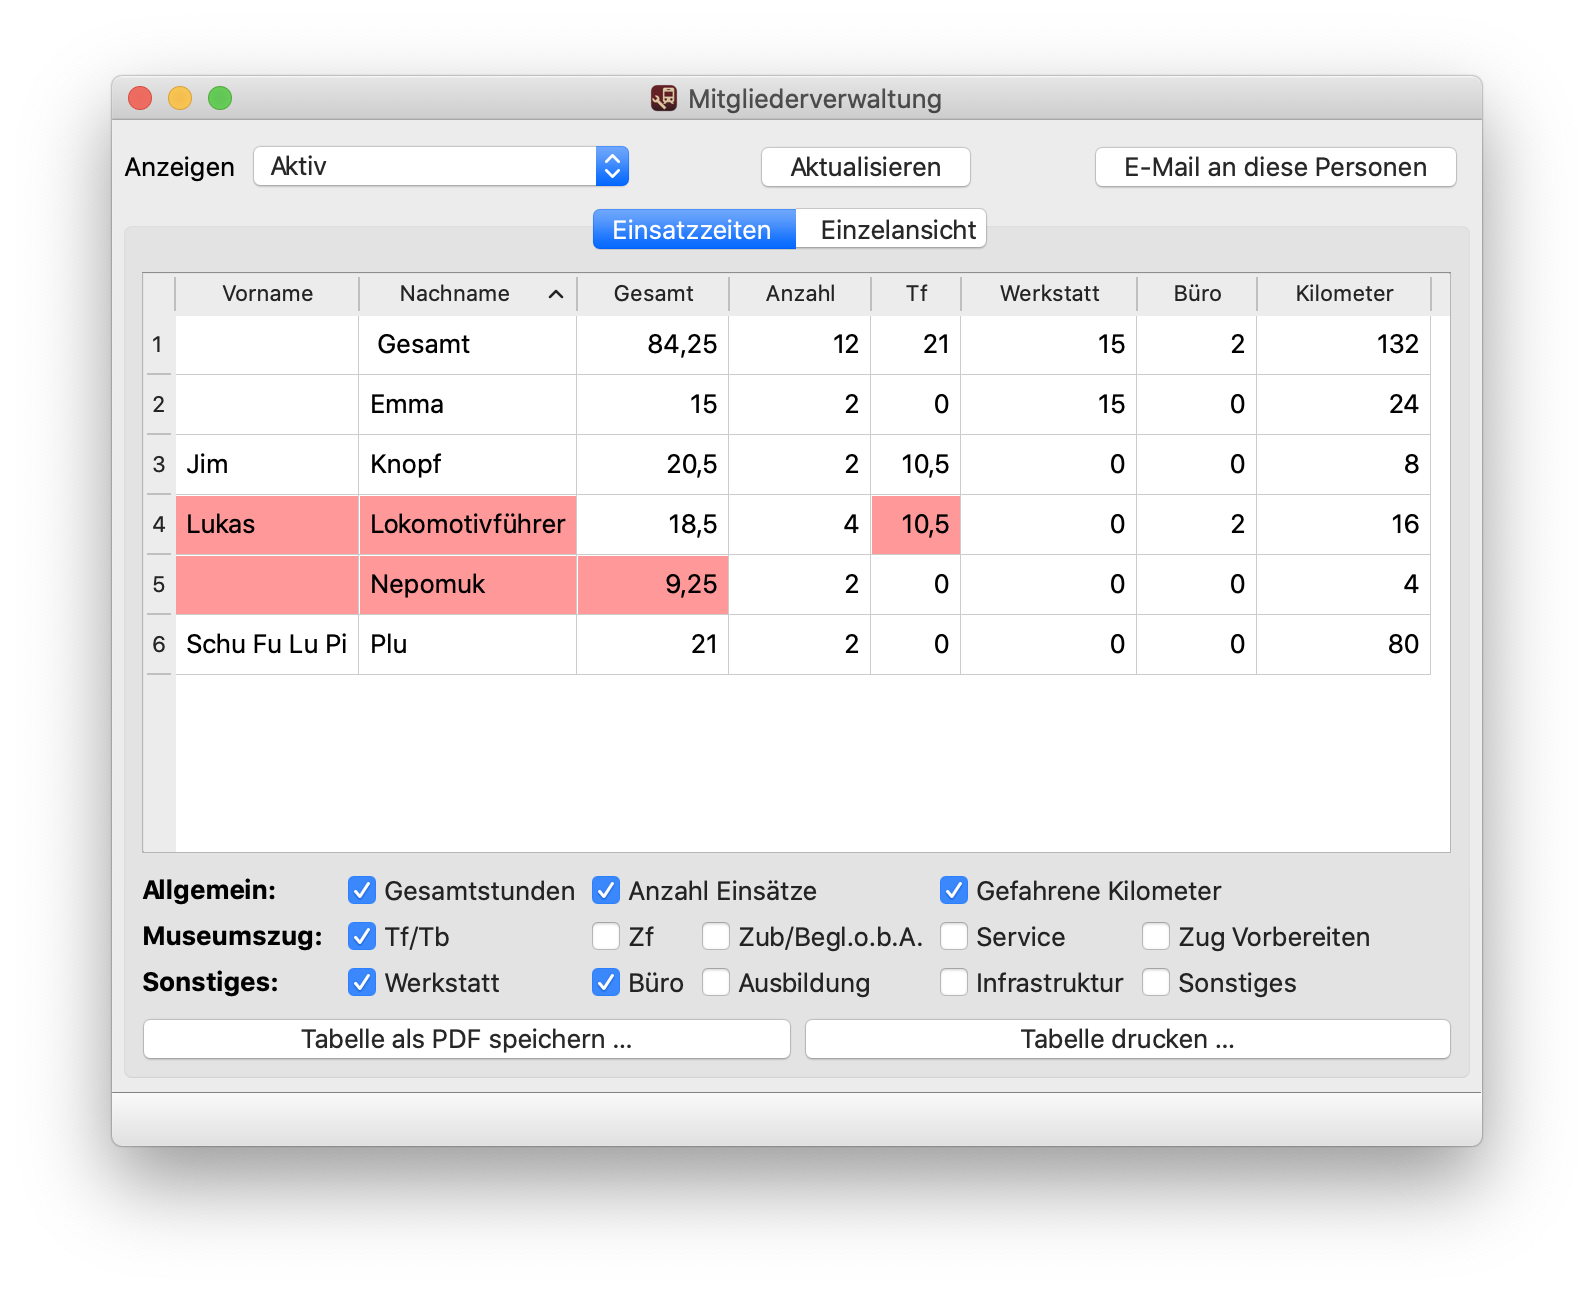
\includegraphics[width=\textwidth]{img/personal_gesamt}
	\caption{Die Personalverwaltung in der Gesamtübersicht.}
	\label{fig:personal:gesamt}
\end{figure}
In der Tabelle von Abbildung~\ref{fig:personal:gesamt} wird eine Übersicht über alle in der Kopfzeile ausgewählten Personen gegeben.
Die Einfärbung erfolgt anhand der mindestens zu erbringenden Stunden.
Rot bedeuted hierbei, dass die Person ihre Stunden noch nicht erbracht hat.
Eine weiße Markierung bestätigt, dass die Mindesstunden erbracht wurden, oder keine solchen gefordert sind (z.B.\ bei passiven Mitglieder).
Passive Mitglieder, die Stunden geleistet haben, werden grün markiert.
Durch einen Doppelklick auf den Eintrag einer Person in der Tabelle wird die entsprechende Einzelansicht geöffnet.


Mit Hilfe der Auswahlkästchen können die verschiedenen Spalten mit den Zeiten der Personen ein- und ausgeblendet werden, die dann auch entsprechend sortiert werden können.
Ebenso wird die Summe der jeweiligen Spalten in der Zeile "`Gesamt"' angegeben.
Diese Zeile ist in der Ausgabe ebenso enthalten.


Mit den Knöpfen "`Tabelle als PDF speichern \dots"' und "`Tabelle drucken \dots"' kann man die Daten der Tabelle exportieren.
Diese Funktionen sind auch im Menü "`Eportieren"' verfügbar.


\paragraph{Mindeststunden}
Die Mindeststunden können über den Eintrag "`Mindeststunden \dots"' im Menü "`Personalmanagement"' bearbeitet werden.
Der sich öffnende Dialog ist in Abbildung~\ref{fig:personal:mindeststunden} dargestellt.

\begin{figure}[!h]
	\centering
	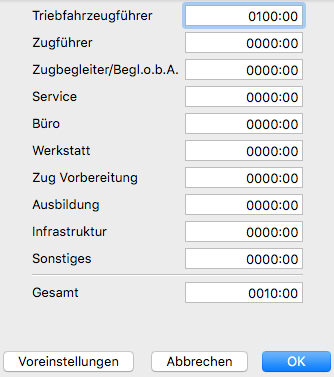
\includegraphics[width=0.5\textwidth]{img/personal_mindeststunden}
	\caption{Der Dialog zum Ändern der Mindesstunden.}
	\label{fig:personal:mindeststunden}
\end{figure}

Standardmäßig sind 10 Stunden für alle aktiven Mitglieder eingestellt.
Personal mit Ausbildung zum Lokführer muss 100 Stunden als Lokführer ableisten.
Die Werte für jedes Konto können beliebig geändert werden.

Die Mindeststunden für Ausbildung werden nur für Personal mit einer betrieblichen Ausbildung und bestehender Tauglichkeit angewendet.




\section{Einzelansicht}\label{personal:einzelansicht}
\begin{figure}[!h]
	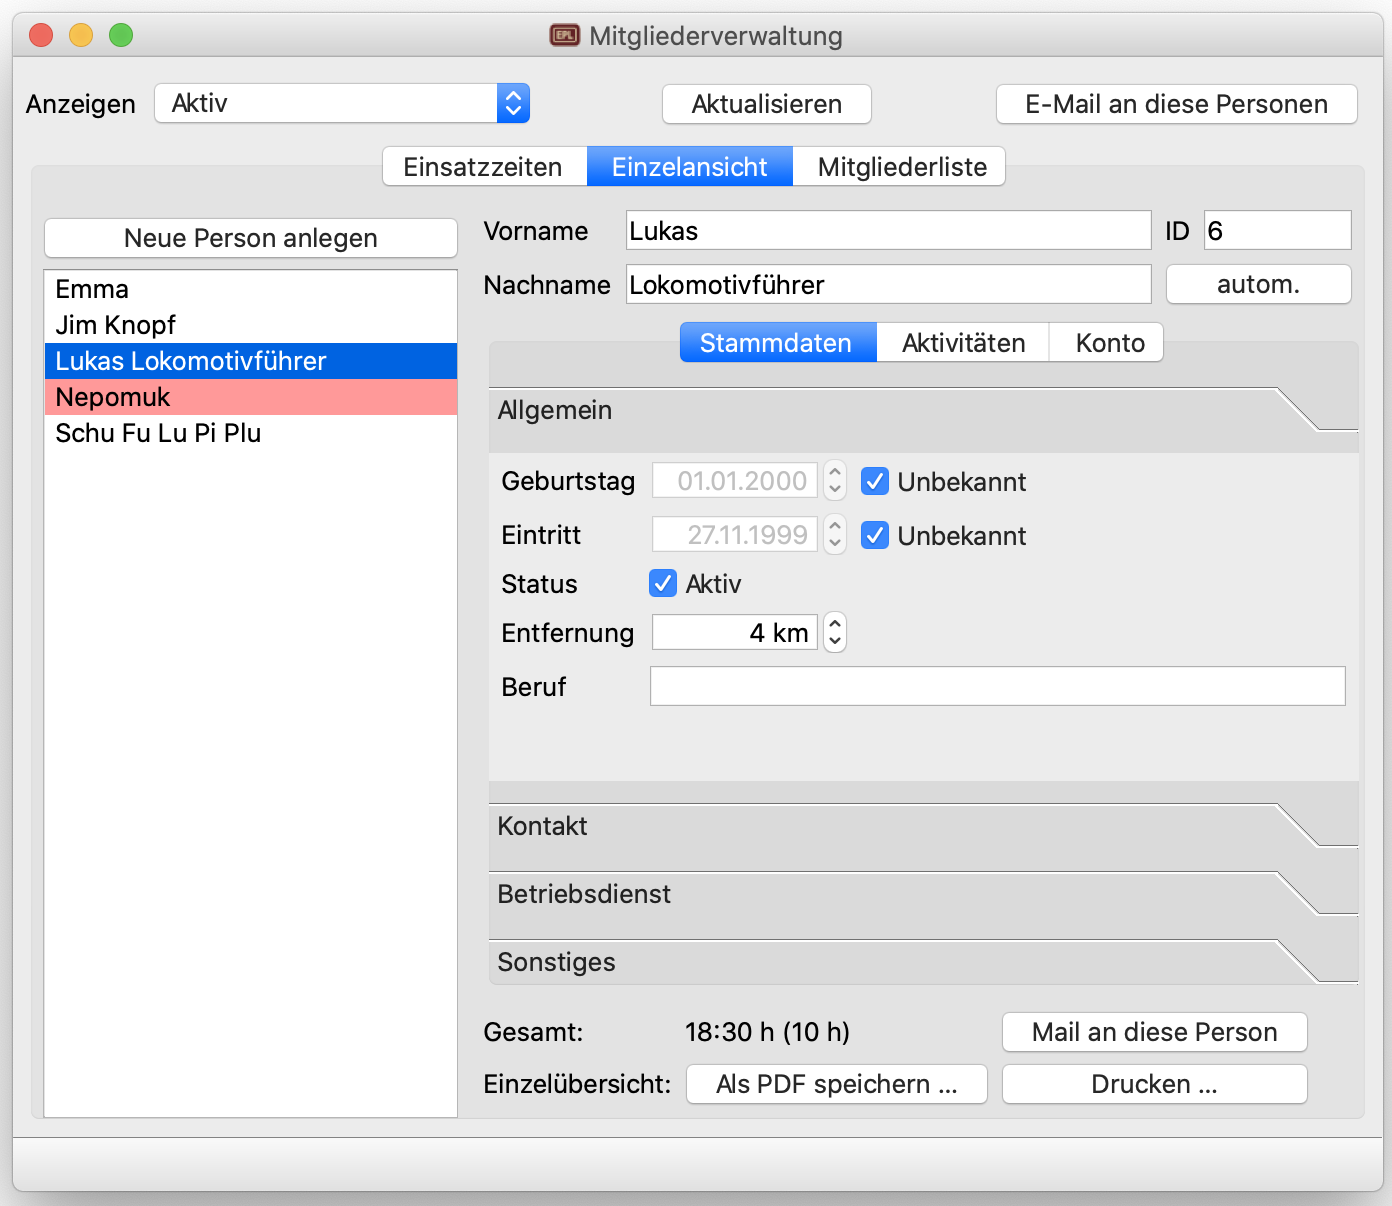
\includegraphics[width=\textwidth]{img/einzelansicht_stammdate_allgemein}
	\caption{Die Einzelansicht mit geöffnetem Reiter für die Stammdaten}
	\label{fig:personal:einzel:stammdaten}
\end{figure}
Das Fenster mit geöffneter Einzelansicht ist in Abbildung~\ref{fig:personal:einzel:stammdaten} zu sehen.
In der Liste sind alle Personen gelistet, die nach der Kopfzeile des Fenster angezeigt werden sollen.
Die farbliche hervorhebung erfolgt analog zur Gesamtübersicht.
Im oberen Teil können der Name und die Mitgliedsnummer der Person verändert werden.
Alternativ zu manuellen Eingabe der Nummer, kann auch eine solche automatisch zugewiesen werden.
Dabei wird die die nächst größere Zahl der aktuell höchsten Mitgliedsnummer verwendet.
Naturgemäß kann eine Nummer nicht doppelt vergeben werden.

Mit den Knöpfen "`Als PDF speichern \dots"' und "`Drucken\dots"' kann eine Übersicht der aktuellen Person ausgegeben werden.
Dort werden dann die Aktivitäten einzeln mit den jeweiligen Zeiten aufgelistet.
Diese Ansicht enthält nur wenige persönliche Informationen.


\paragraph{Stammdaten}
Unter \emph{Allgemein} können das Geburtsdatum, Eintrittsdatum und der Status (Aktiv/Passiv) der Person angegeben werden.
Das Feld "`Entfernung"' wird verwendet die gefahrene Wegstrecke aufgrund der Aktivitäten zu berechnen.
Ebenso kann der erlernte Beruf der Person eingegeben werden.

Unter \emph{Kontakt} besteht die Möglichkeit eine Postadresse, Telefonnummmer und Mailadresse einzutragen.
Ebenso besthet die Möglichkeit anzugebene, ob das Mitglied seine Einwilligung zur Veröffentlichung für Vereinsmitglieder und Betriebsangehörige erteilt hat.

Der Bereich \emph{Betriebsdienst} bietet die Möglichkeit betriebliche Ausbildungen zu erfassen.
Das Feld Tauglichkeit dient dazu anzugeben, bis wann die aktuelle Tauglichkeitsuntersuchung gilt (letzter Tag der Gültigkeit).
Personal, dessen Tauglichkeit nicht mehr gegeben ist, wird wie Personal ohne betriebliche Ausbildung behandelt.

Unter \emph{Sonstiges} gibt es ein Feld für Bemerkungen und die Möglichkeit den Austritt einer Person einzutragen.
Auch kann dort die Person aus dem System entfernt werden.

\hinweis{Eine Person kann erst dann gelöscht werden, wenn Sie in keinen Aktivitäten mehr eingetragen ist.
Siehe nächster Absatz.}


\begin{figure}[!h]
	\centering
	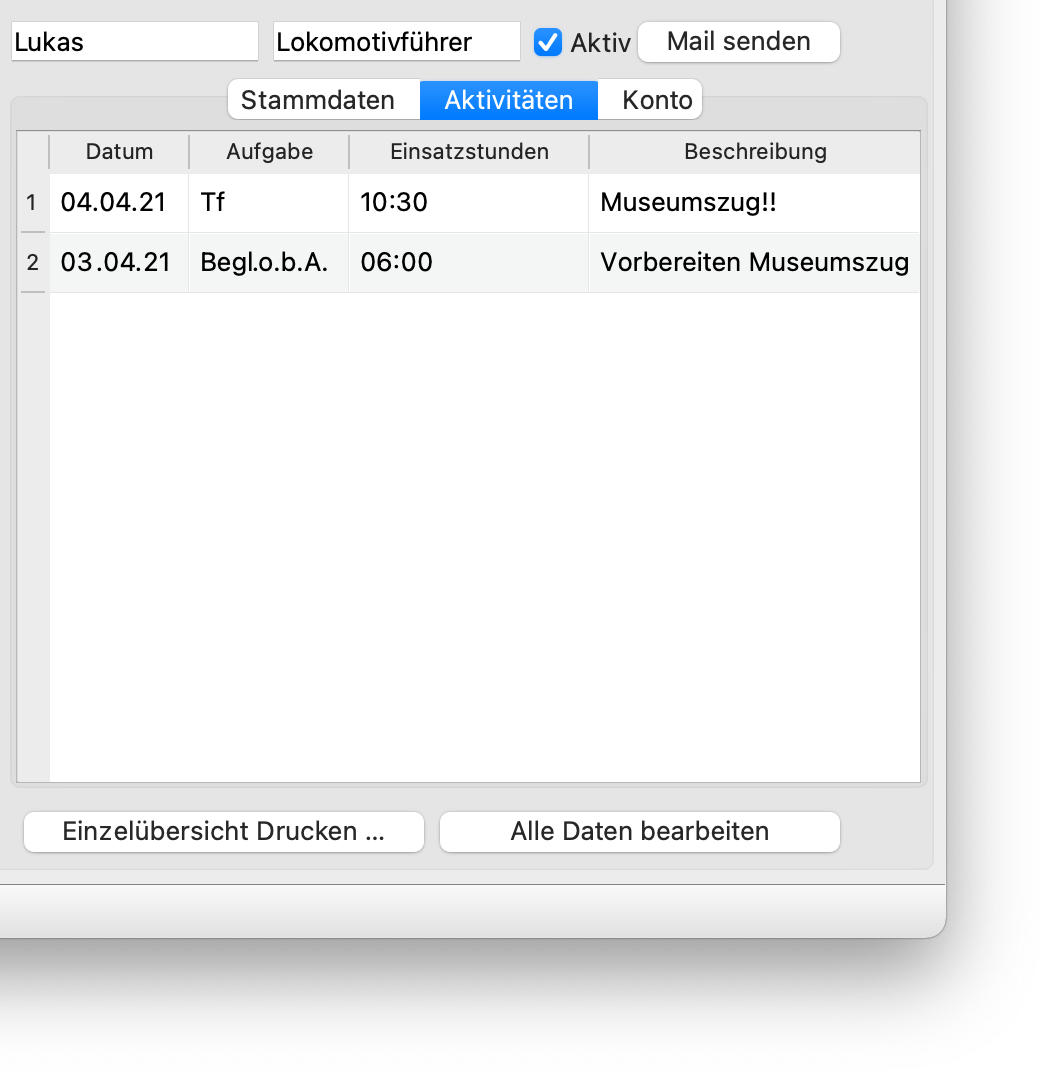
\includegraphics[width=.75\textwidth]{img/einzelansicht_aktivitaeten}
	\caption{Die Einzelansicht mit geöffnetem Reiter für die Aktivitäten}
	\label{fig:personal:einzel:aktivitaeten}
\end{figure}
\paragraph{Aktivitäten}
Der Reiter,
des in Abbildung~\ref{fig:personal:einzel:aktivitaeten} dargestellten Fensters,
zeigt eine Tabelle mit den Aktivitäten,
an denen die ausgewählte Person mitgeholfen hat.


\begin{figure}[!h]
	\centering
	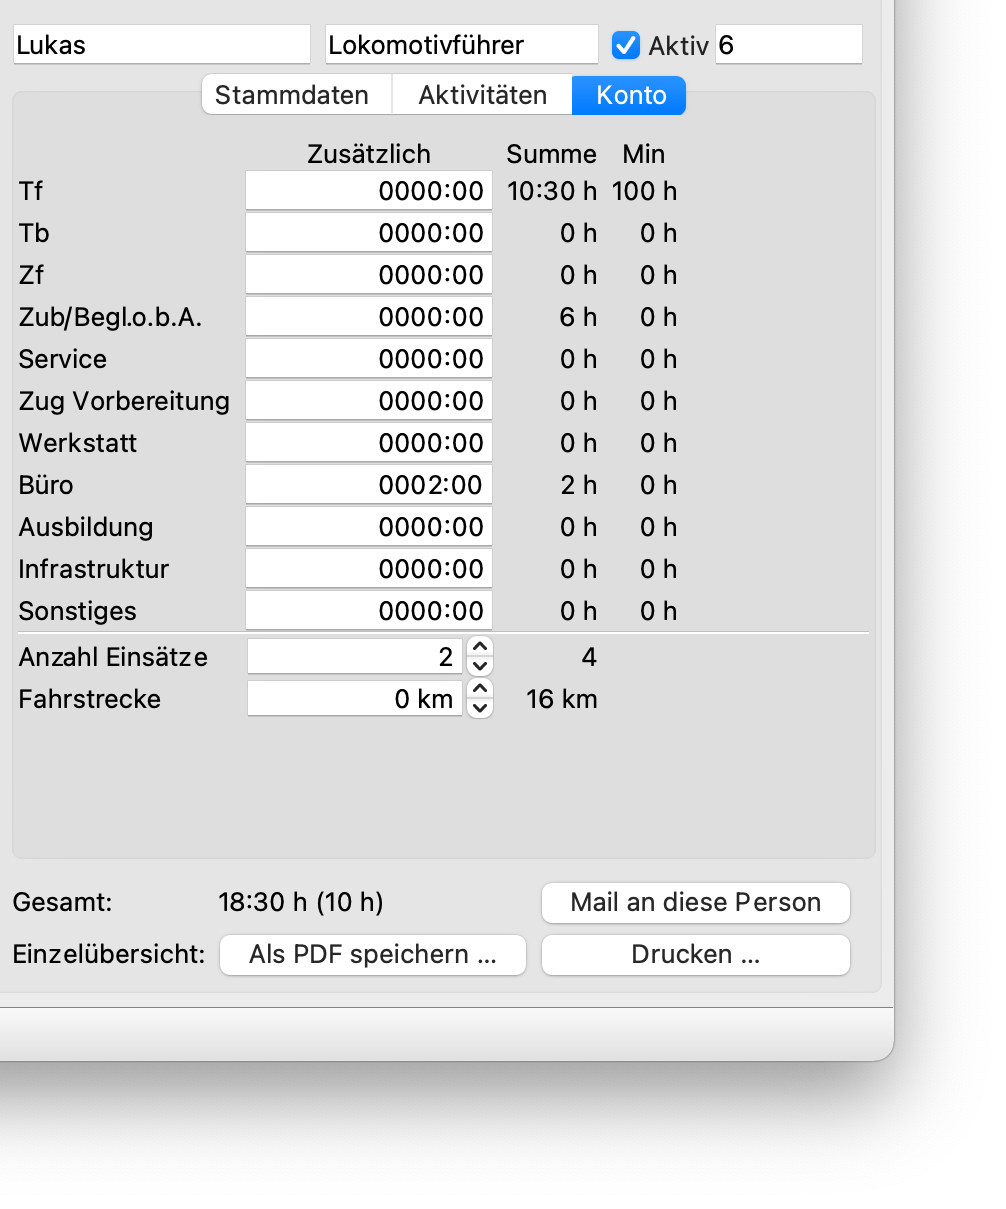
\includegraphics[width=.75\textwidth]{img/einzelansicht_konto}
	\caption{Die Einzelansicht mit geöffnetem Reiter für das Zeitenkonto}
	\label{fig:personal:einzel:konto}
\end{figure}
\paragraph{Konto}
Die Übersicht in Abbildung~\ref{fig:personal:einzel:konto} enthält die Zeiten aufgeteilt nach den verschiedenen Zeit-Konten.
Ebenso können hier zusätzliche Stunden und Kilometer eintragen werden,
welche die Person geleistet hat, aber keiner im System erfassten Aktivität zuzuordnen sind.
Die Anzahl der zusätzlichen Aktivitäten kann ebenfalls erfasst werden.
Ebenso kann man sehen, in welchen Gebieten die Person ihre Pflichtstunden erfüllt hat und wieviele Mindeststunden Sie jeweils in den Gebieten erbringen muss.


\hinweis{Für alle Darstellungen und Berechnungen werden nur die Zeiten angerechnet, die bisher auch wirklich abgeleistet wurden,
also deren Datum in der Vergangenheit lag.}
